\documentclass{beamer}
\usepackage{amsmath}
\usepackage{amssymb}
\usepackage{amsfonts}
\usepackage{bm}

\usepackage{graphicx}
\graphicspath{{./code/figures/}}
\usepackage{hyperref}
\hypersetup{
  colorlinks=true,
  linkcolor=blue,
  filecolor=magenta,
  urlcolor=blue,
}

\usepackage{tikz}
\usepackage{pgfplots}
\pgfplotsset{compat=1.18}

\usetheme{Boadilla}
\usecolortheme{seahorse}

\title{Bayesian Linear Regression}
\author{Vasilis Gkolemis}
\institute{ATHENA RC | HUA}
\date{June 2025}

\begin{document}

% Automatically insert agenda slide at the start of each section
\AtBeginSection[]{
  \begin{frame}{Program}
    \tableofcontents[currentsection]
  \end{frame}
}

\begin{frame}
  \titlepage
  \vfill
  \footnotesize
  \textcopyright\
  Vasilis Gkolemis, 2025. Licensed under CC BY 4.0.
\end{frame}

\begin{frame}{A Synthetic Dataset}
  \begin{itemize}
  \item We will use a synthetic dataset for demonstration.
  \item The dataset is generated using a simple linear function with added Gaussian noise.
  \end{itemize}
  \begin{itemize}
  \item[] \[y = wx + \beta + \epsilon\]
    where:
  \item[] $w = 2$, $\beta = -1$ and $\epsilon \sim \mathcal{N}(0, \sigma^2), \sigma^2 = 1$.
  \item[] $x \sim \mathcal{U}([-3, 3])$ is uniformly distributed.
  \item[] $y$ is the target variable.
    \end{itemize}
  \end{frame}

\begin{frame}{A Synthetic Dataset}
  \begin{itemize}
  \item The dataset $\mathcal{D} = \{(x_i, y_i)\}_{i=1}^{N}$ consists of $N = 100$ samples.
  \end{itemize}
  \begin{center}
    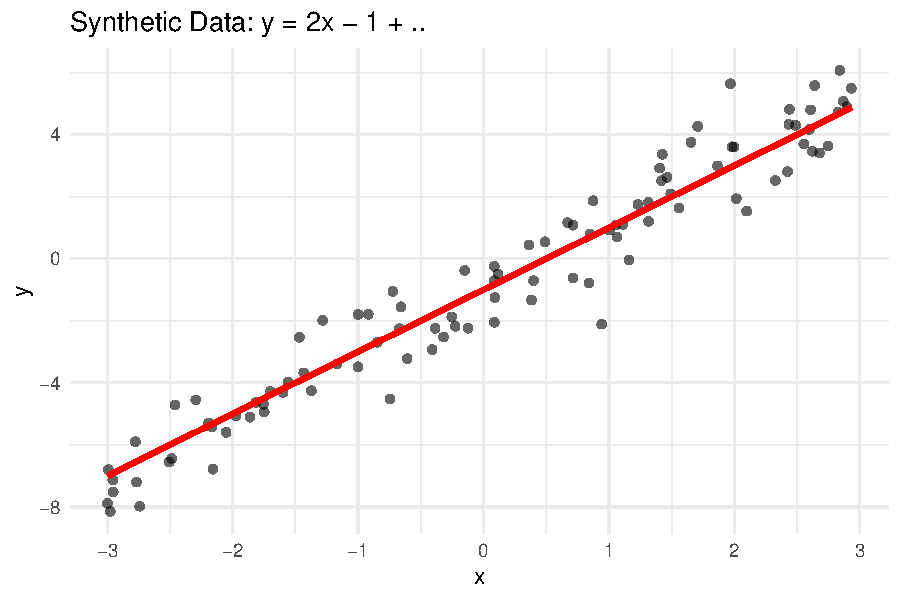
\includegraphics[width=0.7\textwidth]{ground_truth.pdf}
  \end{center}
  \end{frame}


  \section{Prior}

  \begin{frame}{Prior}
    \begin{itemize}
    \item In Bayesian linear regression, we assume a prior distribution over the model parameters.
    \item The prior reflects our beliefs about the parameters before observing any data.
    \item A common choice is a Gaussian prior or a uniform prior.
    \item The prior is denoted as \(p(\bm{\theta})\), where \(\bm{\theta} = (w, b)\) are the parameters of the linear model.
    \end{itemize}
\end{frame}



\begin{frame}{Prior on the parameters}
  \textbf{Prior for slope \(w\) and intercept \(b\):}
  \(
    w, b \sim \mathcal{N}\big(0, 1\big)
  \)

  \begin{center}
    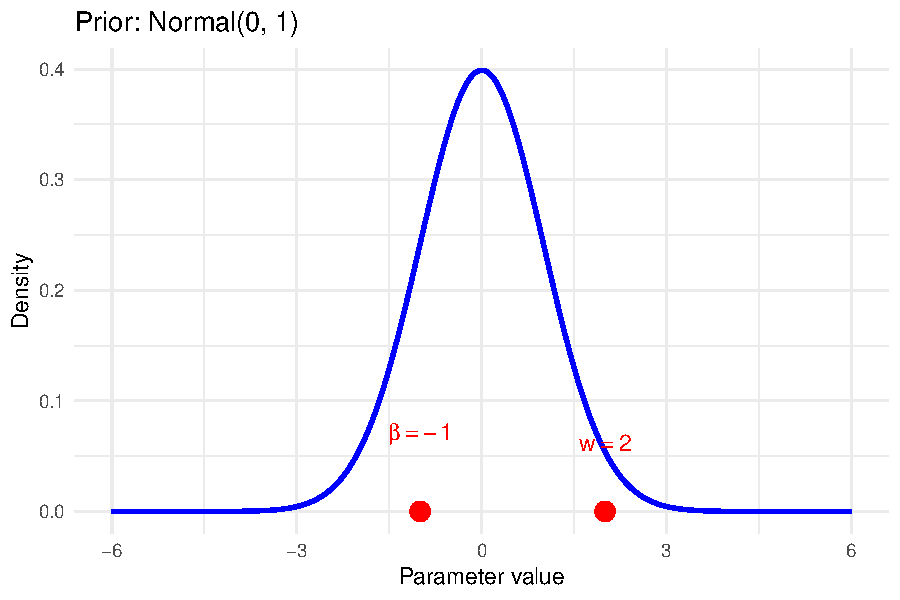
\includegraphics[width=0.8\linewidth]{prior_1_1.pdf}
  \end{center}
\end{frame}

\begin{frame}{Prior on the parameters}
  \textbf{Prior for slope \(w\) and intercept \(b\):}
  \(
    w, b \sim \mathcal{N}\big(0, 1\big)
  \)

  \begin{center}
    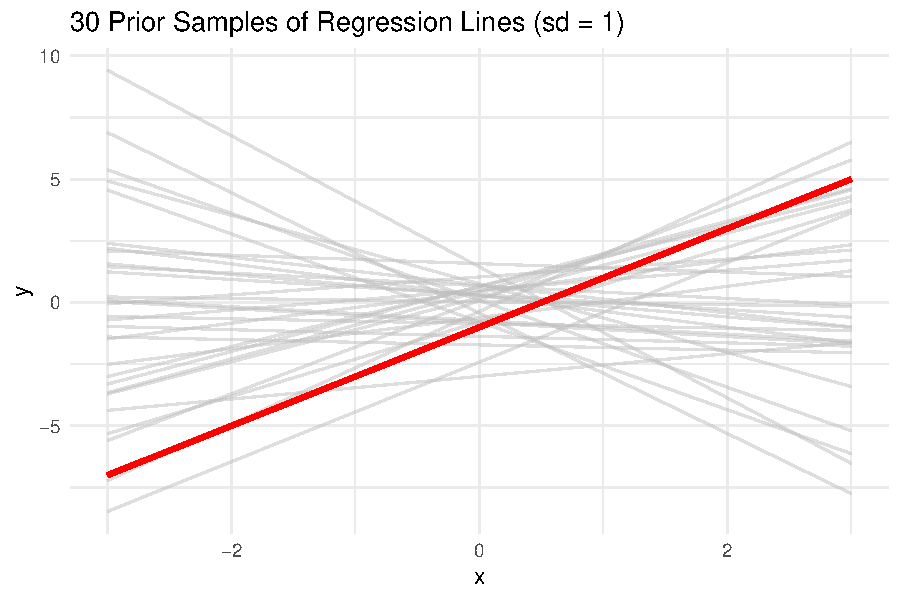
\includegraphics[width=0.8\linewidth]{prior_2_1.pdf}
  \end{center}
\end{frame}

% Slide 2: Wider Prior
\begin{frame}{Prior with Larger Variance (Less Informative)}
  Increasing the prior variance expresses less certainty about \(w, b\):
  \(
    w, b \sim \mathcal{N}\big(0, 4\big)
  \)

  \begin{center}
    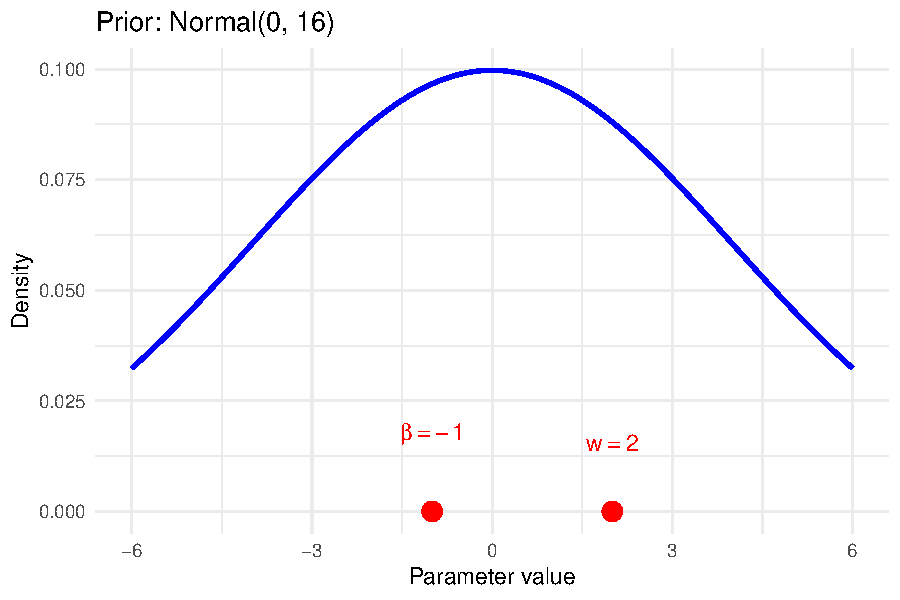
\includegraphics[width=0.8\linewidth]{prior_1_2.pdf}
  \end{center}
\end{frame}

\begin{frame}{Prior with Larger Variance (Less Informative)}
  Increasing the prior variance expresses less certainty about \(w, b\):
  \(
    w, b \sim \mathcal{N}\big(0, 4\big)
  \)

  \begin{center}
    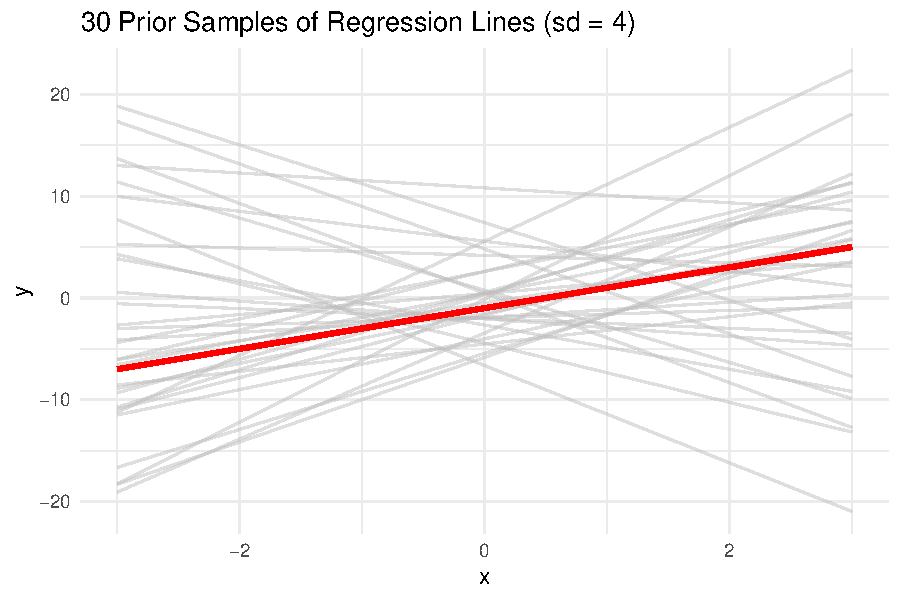
\includegraphics[width=0.8\linewidth]{prior_2_2.pdf}
  \end{center}
\end{frame}

% Slide 3: Incorrect Prior (Excluding Ground Truth)
\begin{frame}{Incorrect Prior that Excludes True Parameters}
  A poorly chosen prior far from the truth, with low variance:
  \(
    w, b \sim \mathcal{N}\big(0, 0.4\big)
  \)


  \begin{center}
    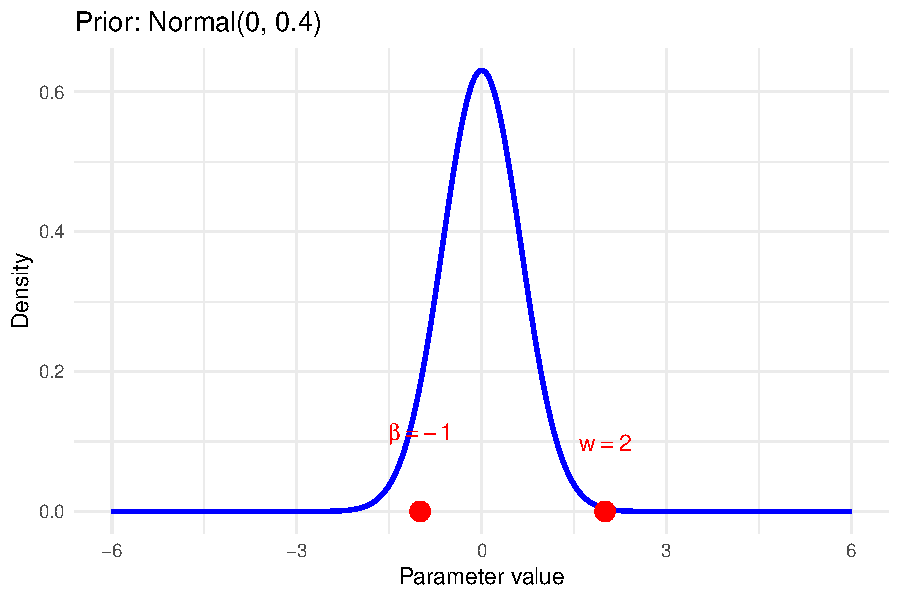
\includegraphics[width=0.8\linewidth]{prior_1_3.pdf}
  \end{center}
\end{frame}

\begin{frame}{Incorrect Prior that Excludes True Parameters}
  A poorly chosen prior far from the truth, with low variance:
  \(
    w, b \sim \mathcal{N}\big(0, 0.4\big)
  \)

  \begin{center}
    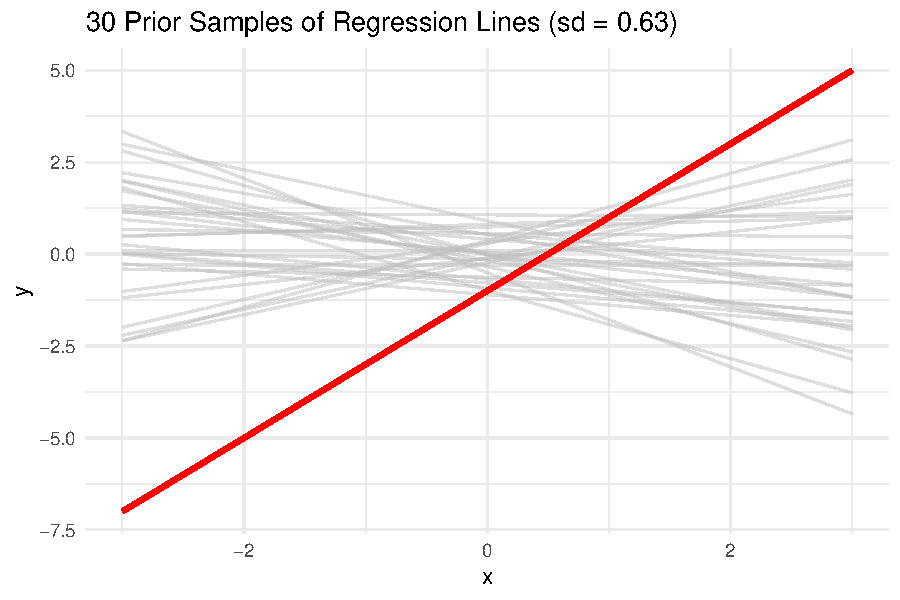
\includegraphics[width=0.8\linewidth]{prior_2_3.pdf}
  \end{center}
\end{frame}

\section{Posterior}

\begin{frame}{Posterior}
  \begin{itemize}
  \item The posterior distribution combines the prior and the likelihood of the observed data.
  \item It is computed using Bayes' theorem:
    \[
      p(\bm{\theta} | \mathcal{D}) \propto p(\mathcal{D} | \bm{\theta}) p(\bm{\theta})
                                   \propto p(\bm{\theta}) \prod_{i=1}^{N} p(y^i | x^i, \bm{\theta})
  \]

  \item The posterior reflects our updated beliefs about the parameters after observing the data.
  \end{itemize}
\end{frame}

\begin{frame}{Posterior}
  We can compute the posterior in analytic form for linear regression with Gaussian noise:
  \begin{itemize}
  \item The posterior distribution is also Gaussian:
    \[
      p(\bm{\theta} | \mathcal{D}) = \mathcal{N}(\bm{\mu}, \bm{\Sigma})
    \]
  \item The posterior mean \(\bm{\mu}\) and covariance \(\bm{\Sigma}\) can be computed as:
    \[
      \bm{\mu} = (\bm{X}^T \bm{X} + \sigma^2 \bm{I})^{-1} \bm{X}^T \bm{y}
    \]
    \[
      \bm{\Sigma} = (\bm{X}^T \bm{X} + \sigma^2 \bm{I})^{-1}
    \]
  \item Skip the maths for now!
  \end{itemize}

\end{frame}

\begin{frame}{Posterior}
  \textbf{Posterior when prior was \(\mathcal{N}(0, \sigma^2=1)\):}
  \(
    w, b | \mathcal{D} \sim \mathcal{N}\big(\bm{\mu}, \bm{\Sigma}\big)
  \)

  \begin{center}
    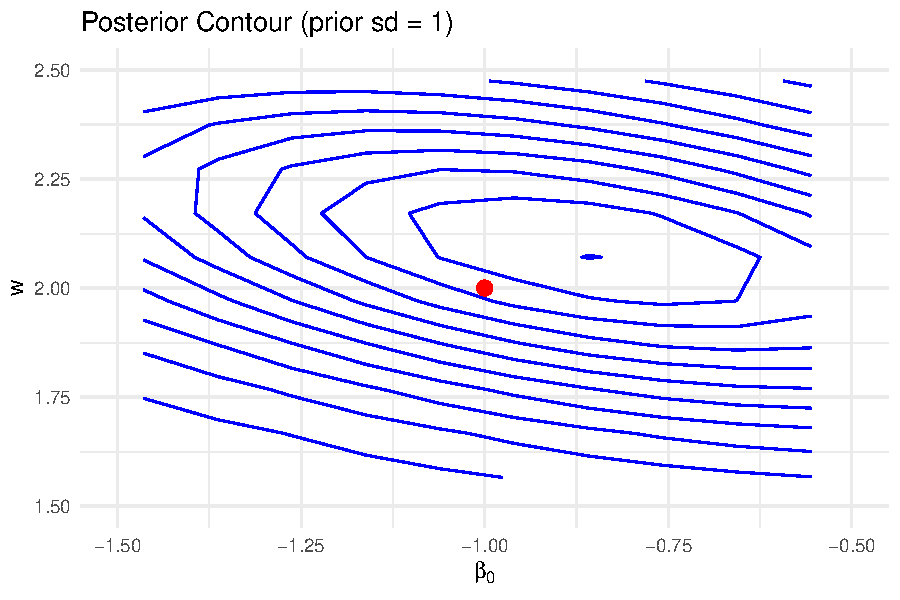
\includegraphics[width=0.8\linewidth]{posterior_contour_1.pdf}
  \end{center}
\end{frame}

\begin{frame}{Posterior}
  \textbf{Posterior when prior was \(\mathcal{N}(0, \sigma^2=1)\):}

  \begin{center}
    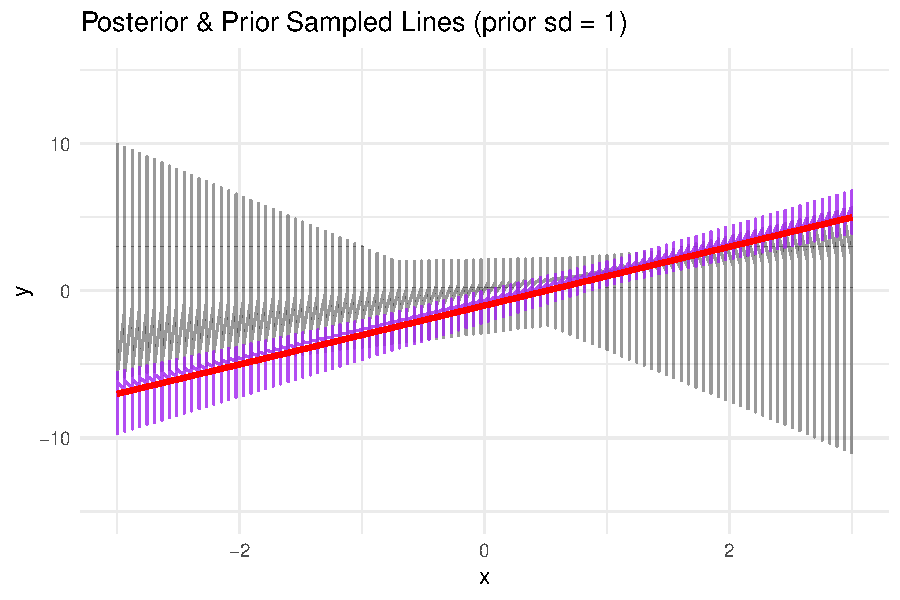
\includegraphics[width=0.8\linewidth]{posterior_lines_1.pdf}
  \end{center}
\end{frame}

\begin{frame}{Posterior}
  \textbf{Posterior when prior was \(\mathcal{N}(0, \sigma^2=4)\):}

  \begin{center}
    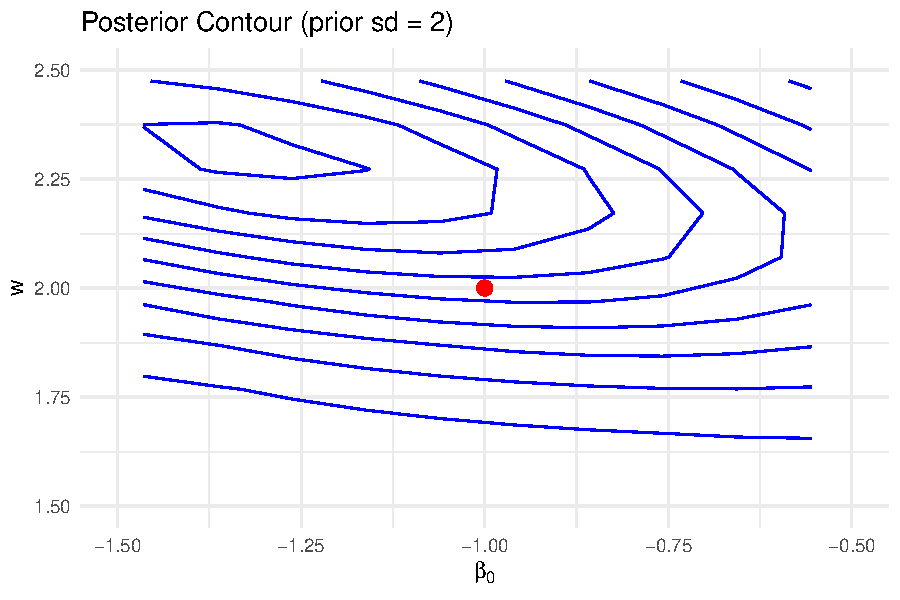
\includegraphics[width=0.8\linewidth]{posterior_contour_2.pdf}
  \end{center}
\end{frame}

\begin{frame}{Posterior}
  \textbf{Posterior when prior was \(\mathcal{N}(0, \sigma^2=4)\):}

  \begin{center}
    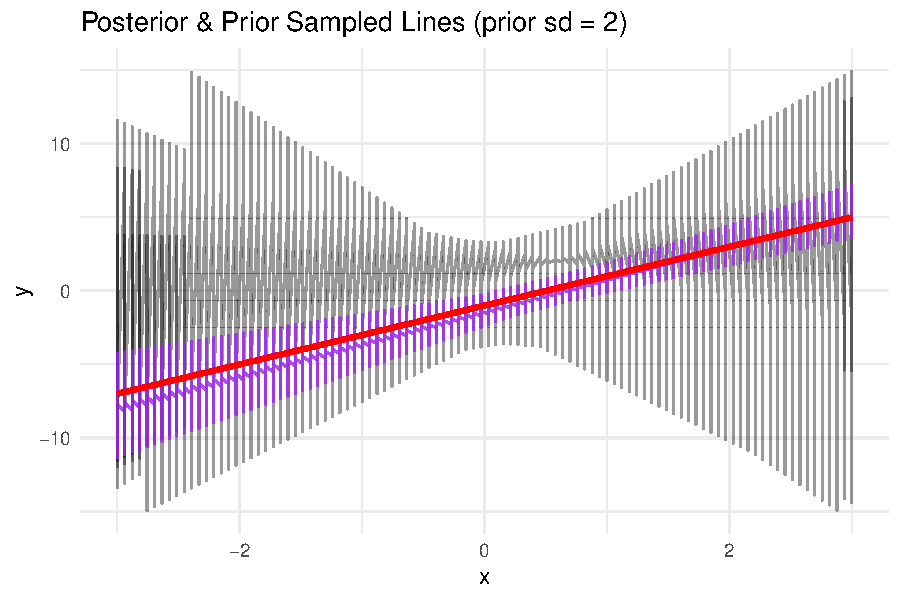
\includegraphics[width=0.8\linewidth]{posterior_lines_2.pdf}
  \end{center}
\end{frame}

\begin{frame}{Posterior}
  \textbf{Posterior when prior was \(\mathcal{N}(0, \sigma^2=0.4)\):}

  \begin{center}
    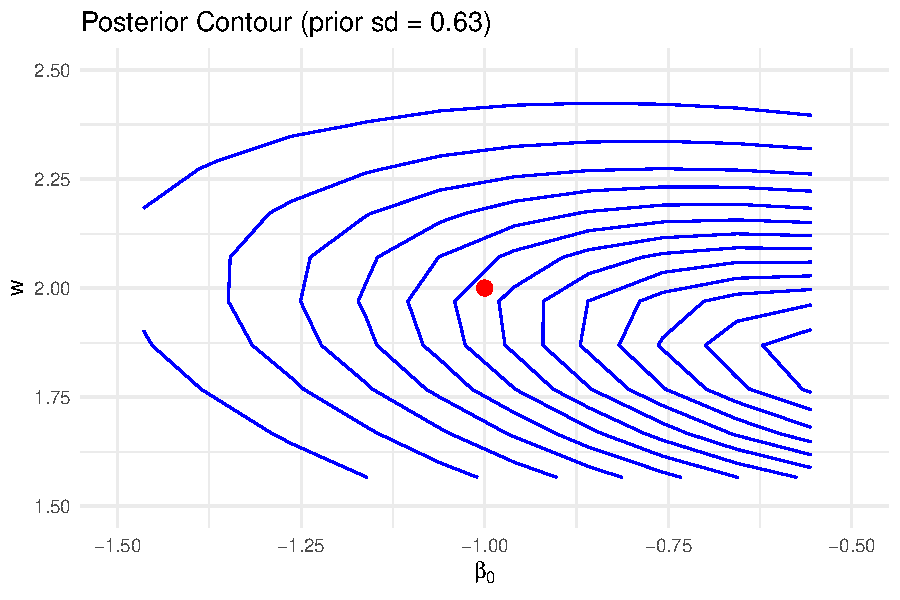
\includegraphics[width=0.8\linewidth]{posterior_contour_3.pdf}
  \end{center}
\end{frame}

\begin{frame}{Posterior}
  \textbf{Posterior when prior was \(\mathcal{N}(0, \sigma^2=0.4)\):}

  \begin{center}
    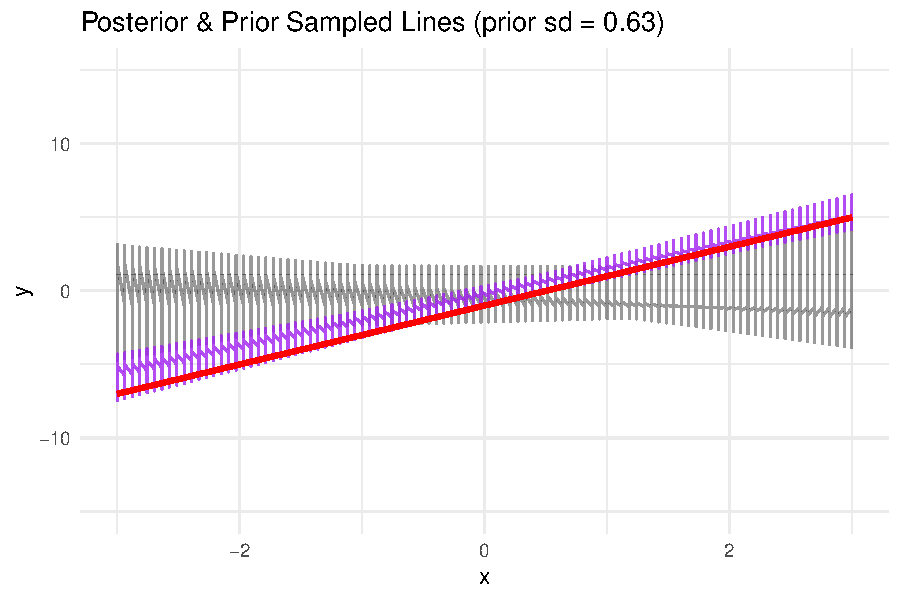
\includegraphics[width=0.8\linewidth]{posterior_lines_3.pdf}
  \end{center}
\end{frame}

\begin{frame}{Summary}
  \begin{itemize}
  \item Surprisingly (?), the posterior is accurate even when the prior does not match the true parameters.
  \item The posterior is influenced by the prior, but the data (likelihood) has a strong effect.
  \item However, do not be that overconfident!
  \item Our example is simple, and the prior is Gaussian which has infinite support.
  \item If the prior was a uniform distribution, i.e., $\mathcal{U}([-1, 1])$, with the true parameters outside this range, Bayesian linear regression would fail to learn the true parameters.
  \end{itemize}
\end{frame}

\begin{frame}{Summary}
  \begin{itemize}
  \item Surprisingly (?), the posterior is accurate even when the prior does not match the true parameters.
  \item The posterior is influenced by the prior, but the data (likelihood) has a strong effect.
  \item However, do not be that overconfident!
  \item Our example is simple, and the prior is Gaussian which has infinite support.
  \item Even with fewer data points, $N=3$, the posterior becomes worse if the prior is not informative enough.
  \end{itemize}
\end{frame}
\begin{frame}{Posterior with $N=5$}

  \only<1>{
    \textbf{Posterior when prior was \(\mathcal{N}(0, \sigma^2=1)\) and $N=5$}
    \begin{center}
      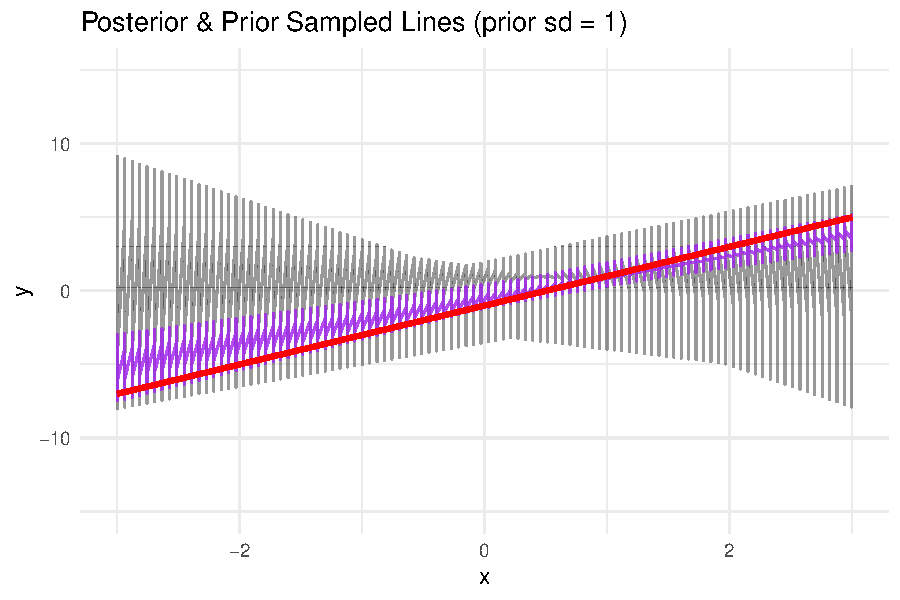
\includegraphics[width=0.8\linewidth]{posterior_lines_less_1.pdf}
    \end{center}
  }

  \only<2>{
    \textbf{Posterior when prior was \(\mathcal{N}(0, \sigma^2=4)\) and $N=5$}
    \begin{center}
      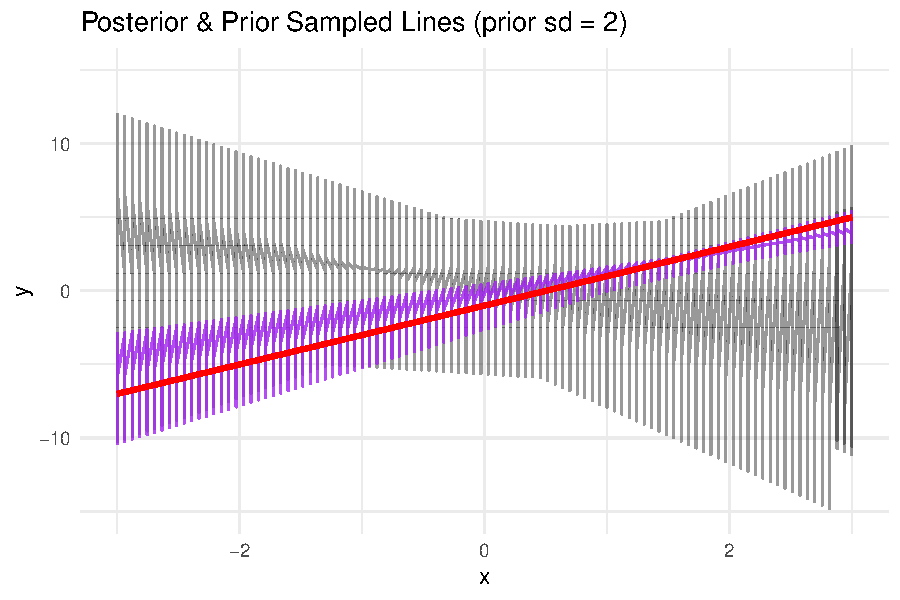
\includegraphics[width=0.8\linewidth]{posterior_lines_less_2.pdf}
    \end{center}
  }

  \only<3>{
    \textbf{Posterior when prior was \(\mathcal{N}(0, \sigma^2=0.4)\) and $N=5$}
    \begin{center}
      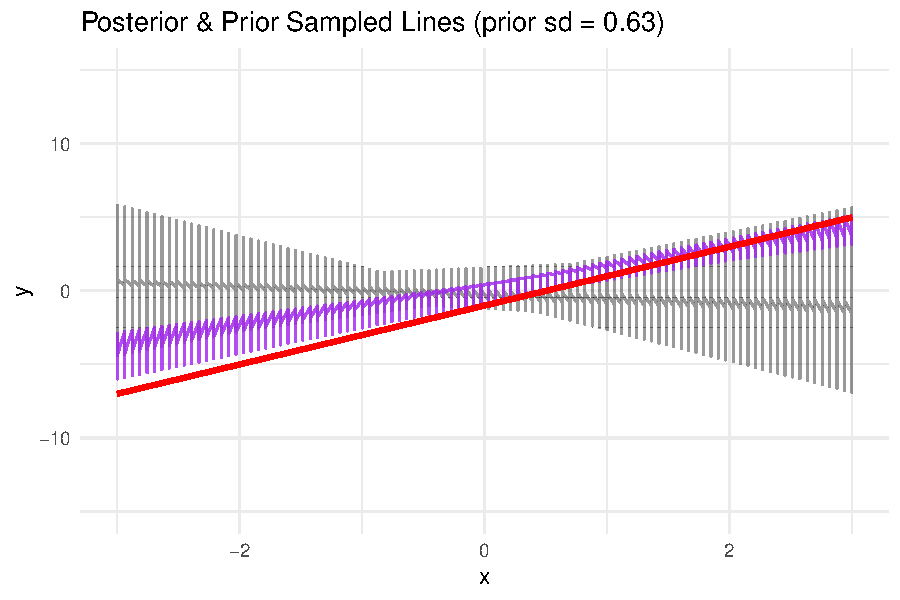
\includegraphics[width=0.8\linewidth]{posterior_lines_less_3.pdf}
    \end{center}
  }

\end{frame}


\section{Conjugate Priors}


\begin{frame}{Conjugate Priors: Motivation}
  \begin{itemize}
    \item In Bayesian inference, we update our belief (the prior) after seeing data (via the likelihood) to get the posterior:
      \[
        p(\bm{\theta} | \mathcal{D}) \propto p(\mathcal{D} | \bm{\theta}) \cdot p(\bm{\theta})
      \]
    \item In general, computing this posterior is hard—often requires numerical methods (e.g., MCMC, variational inference).
    \item But in some special cases, we get a \textbf{closed-form} posterior.
    \item These special cases arise when the \textbf{prior is conjugate to the likelihood}
  \end{itemize}
\end{frame}

\begin{frame}{Definition: Conjugate Prior}
  \begin{block}{Definition}
    A prior is said to be \textbf{conjugate} to the likelihood if the posterior is in the same family as the prior.
  \end{block}
  \begin{itemize}
    \item Example: Gaussian likelihood + Gaussian prior $\Rightarrow$ Gaussian posterior
    \item This allows efficient inference—no need for numerical approximations.
    \item Conjugate priors are available for many common likelihoods:
      \begin{itemize}
        \item Binomial likelihood → Beta prior
        \item Poisson likelihood → Gamma prior
        \item Gaussian likelihood → Gaussian prior (as we'll see!)
      \end{itemize}
  \end{itemize}
\end{frame}

\begin{frame}{Conjugate Prior for Linear Regression}
  \begin{itemize}
    \item Suppose a Bayesian linear regression model:
      \[
        \bm{y} = \bm{X}\bm{\theta} + \bm{\epsilon}, \quad \bm{\epsilon} \sim \mathcal{N}(0, \sigma^2 \bm{I})
      \]
    \item Prior: \( \bm{\theta} \sim \mathcal{N}(0, \sigma^2 \bm{I}) \)
    \item Likelihood: \( p(\bm{y} | \bm{\theta}) = \mathcal{N}(\bm{X}\bm{\theta}, \sigma^2 \bm{I}) \)
    \item Posterior is also Gaussian:
      \[
        p(\bm{\theta} | \bm{y}, \bm{X}) = \mathcal{N}(\bm{\mu}, \bm{\Sigma})
      \]
      with:
      \[
        \bm{\mu} = (\bm{X}^T \bm{X} + \sigma^2 \bm{I})^{-1} \bm{X}^T \bm{y}, \quad
        \bm{\Sigma} = (\bm{X}^T \bm{X} + \sigma^2 \bm{I})^{-1}
      \]
    \end{itemize}
    \begin{itemize}
    \item Proofs can be found in many Bayesian textbooks, e.g., "Bayesian Data Analysis" by Gelman et al.
    \item{Intuition:} The product of Gaussian distributions is another Gaussian.
      \end{itemize}
\end{frame}

\begin{frame}{Why Conjugacy Matters}
  \begin{itemize}
    \item \textbf{Fast, exact inference:} No sampling or approximation needed.
    \item \textbf{Analytic tractability:} Makes teaching, derivation, and understanding easier.
    \item \textbf{Limitations:}
      \begin{itemize}
        \item Only available for limited combinations of priors and likelihoods.
        \item Sometimes the conjugate prior may not reflect real prior beliefs well.
      \end{itemize}
    \item In most real-world cases: we rely on approximate inference.
    \item But conjugacy gives insight into the Bayesian machinery in clean, solvable cases.
  \end{itemize}
\end{frame}

\begin{frame}{Summary}
  \begin{itemize}
    \item What we have learned:
  \begin{itemize}
    \item Bayesian linear regression allows us to incorporate prior beliefs about parameters.
    \item The posterior distribution combines prior and likelihood, updating our beliefs after observing data.
    \item Conjugate priors provide a powerful framework for efficient inference in Bayesian models.
    \end{itemize}
  \item What comes next:
    \begin{itemize}
    \item The world is not linear.
    \item Bayesian linear regression is a starting point, but real-world data often requires more complex models.
    \item In the next two lectures, we will explore how to perform Bayesian inference in more complex models:
      \begin{itemize}
        \item Non-linear regression
        \item Bayesian neural networks
        \end{itemize}
      \end{itemize}
  \end{itemize}
\end{frame}


\end{document}
